\documentclass[11pt, fullpage,letterpaper]{article}
\usepackage{graphicx} % Required for inserting images
\setlength{\parskip}{\baselineskip}%
\setlength{\parindent}{0pt}%
\usepackage[margin=1in]{geometry}
\usepackage{url}
\usepackage{amsmath}
\usepackage{amssymb}
\usepackage{amsfonts}
\usepackage{dsfont}
\usepackage{xspace}
\usepackage{graphicx}
\usepackage{hyperref}
\bibliographystyle{apa}

\title{Probabilistic Machine Learning - Project Final Report}
\author{Matthew Lowery, Ramansh Sharma}
\date{}

% A brief introduction to the problem you want to solve using probabilistic learning techniques.(10%)

% -- operator learning is ___ vs traditional methods
% -- usually done in supervised settings, not unsupervised
% -- generative models are unsupervised, 
%         probabilistic such that, 
%         which are helpful here bc
% -- We focus on VAEs in particular, VANO paper has no code

% The motivation - why do you want to use learning techniques? Why not the traditional or existing methods? (10%)

% --Traditional methods would be? PCA? POD? Kernel-based PCA/POD?
% --


% What you have done to reach your goal. Note that just “We collected data” will NOT be enough (40%)




% What is your detailed plan for the rest of the project (30%)

% 
% 
%

% Reference to literature (10%)


\begin{document}

\maketitle

\section{Introduction}

Operator learning has emerged as a way to parameterize a map between infinite dimensional function spaces, versus usually aiming to learn a map between finite dimensional vector spaces like in traditional neural networks. To learn an operator in essence is to approximate an integral transformation or an integration kernel and apply said `operator' to a discretized input function. The current state-of-art method for doing so works by parameterizing a convolution operator defined in Fourier space, coined the Fourier Neural Operator (FNO; \cite{li2021fourier}), or more simply put, works by manipulating the input function via a manipulation of its Fourier weights. Another prominent method such as DeepONet \cite{Lu_2021} works by learning both basis functions and the coefficients along the basis for the output functions using a neural network (in the form of multilayer perceptrons for 1D problems, and CNN for the branch when the input functions are sampled on a 2D grid).

On the other hand, Variational Autoencoders (VAEs; \cite{kingma2022autoencoding}) are popular unsupervised, generative models that use neural networks in an attempt to reduce finite-dimensional input data to a lower dimensional latent space, wherin this latent space is prescribed as a probability measure. In practice this entails having an encoding MLP that maps an input to two vectors, which parameterize $\mathbf{\mu}$ and the diagonal of $\mathbf{\Sigma}$ a multivariate Gaussian, sampling from that Gaussian in a backprop-able way, and having another decoding MLP attempt reconstruct the input function. The benefit of VAEs is (1) that the latent space can be sampled from to generate new data and (2) that the data dimensionality is significantly reduced.

Recently, the Variational Neural Operator (VANO; \cite{seidman2023variational}) was introduced to make VAEs amenable with functional data. This means that the latent space representation now becomes a distribution of output functions to sample from, and by proxy, a distribution of operators applied to the input function to sample from. A lot of progress has been made for operator learning frameworks for supervised learning problems as opposed to unsupervised problems. Unsupervised problems are interesting in modeling physical systems and partial differential equations (PDEs) because of the natural lack of large datasets in these problems. In this regard, VANO brings many advantages by introducing a novel encoder-decoder architecture for dimensionality reduction and generative modeling of functional data. Our goal for this project is to write a well documented codebase for this model for numerous 1D and 2D operator learning datasets (including Burgers, Advection, cavity flow, and Darcy flow) as the original work did not release any code. Borrowing notation from the paper, the encoding map $\mathcal{E}(u): u \rightarrow \mathbb{R}^n, \; u \sim \mathcal{X}$, maps an input function $u$ to a latent $n$-dimensional vector. The decoding map maps the latent space to a function $\mathcal{Y}$ that can be evaluated in its domain; $\mathcal{D}: \mathbb{R}^n \rightarrow \mathcal{Y}$.

\section{Motivation}
The operator learning problem involves learning an approximation map between a given set of input and output functions \cite{Lu_2021, fair_paper} which can then be evaluated on previously unseen examples of functions. While machine learning techniques are readily useful with a large variety of architectures for this problem, more traditional scientific computing techniques are not. Non-learning techniques such as principal component analysis (PCA) and proper orthogonal decomposition (POD) are by themselves not expressive enough for large scale datasets or difficult operator learning problems (ones that involve mix of global/local information in the PDE, oscillatory problems, etc.). However, these techniques are useful in unsupervised models such as variational autoencoding neural operators (VANO) \cite{seidman2023variational}.

Without loss of generality, we describe the operator learning problem here. Let $U=\{u_i\}_{i=0}^{N_u}$ and $V=\{v_j\}_{j=0}^{N_v}$ be two sets of functions. The operator $\tilde{G}: \mathcal{U} \rightarrow \mathcal{V}$ is the continuous operator where $u \sim \mathcal{U}$ and $v \sim \mathcal{V}$. Discretely, let $u: \mathbb{R}^{d_1} \rightarrow \mathbb{R}^{d_2}$ be an input function and $x \in \mathbb{R}^{d_1}$ and $y \in \mathbb{R}^{q}$ be points where $d_{1}, d_2, q \in \mathbb{N}$. While it is not necessarily true, the output function $v$ is usually also a map as such $v: \mathbb{R}^{d_1} \rightarrow \mathbb{R}^{d_2}$. Using a machine learning method, one then approximates the operator $G: U \rightarrow V$ by optimizing parameters with a loss function.

\section{Progress}


% -- researched project, understood math, etc
% --  written code for standard VAE as a precursor
% -- used & have worked with other operator models (fno, deep o)
% -- collected other datasets

\subsection{VANO}

For this project, we have meticulously understood the VANO paper, its motivations and mathematical foundations. The core idea behind VANO is to learn an identity map which learns finite dimensional coordinates for the data manifold. The dataset to the model is viewed as coming from a generative model on the coordinate space of the problem, and the model is trained with an auto-encoding Bayes approach. Once trained, the decoder component of the network can generate new functions in the latent coordinate space which can be evaluated anywhere in their domain (in as many spatial or temporal dimensions). The model prevents overfitting at higher data resolutions by making the variational objective \textit{discretization agnostic} with the use of functional data space instead of the space of pointwise evaluations. Fig \ref{fig:vano}, borrowed from the paper, shows the encoder and decoder transformations on a function.

Next, we describe the implementation progress.

\subsection{Code}

We have thus far implemented standard VAEs as a helpful precursor to coding VANO. In adddition, we have implementations of standard operator learning models such as DeepOnet and FNO ready, which we will compare VANO against. 

\subsection{Dataset}
\label{sec:dataset}

We have also collected and made ready the following Operator learning benchmark datasets from \cite{fair_paper}:

\begin{enumerate}
    \item Burgers
        \begin{align}
            \frac{\partial u}{\partial t} + u \frac{\partial u}{\partial x} = \nu \frac{\partial^2 u}{\partial x^2}, x \in (0, 1), t \in (0, 1].
        \end{align}

    \item Advection
        \begin{align}
            \frac{\partial u}{\partial t} + \frac{\partial u}{\partial x} = 0, x \in [0, 1], t \in [0, 1].
        \end{align}

    \item Regularized cavity flow
        \begin{align}
            \nabla \cdot u = 0, \nonumber \\
            \partial_t u + u \cdot \nabla u = - \nabla P + \nu \nabla^2 u,
        \end{align}

        where $u$ is a 2D or 3D field depending on the problem.

    \item Darcy flow
        \begin{align}
            - \nabla \cdot (K(x, y) \nabla h(x, y)) = f, \; (x, y) \in \Omega,
        \end{align}

        where $K$ is the permeability field, $h$ is the pressure, and $f$ is a source term which can either be a constant or a space-dependent function. \textbf{Note}: Darcy flow has 4 variations, (1) rectangular domain with continuous permeability field, (2) rectangular domain with piecewise constant permeability field, (3) triangular domain, and (4) triangular domain with a notch.
\end{enumerate}

\begin{figure}
    \centering
    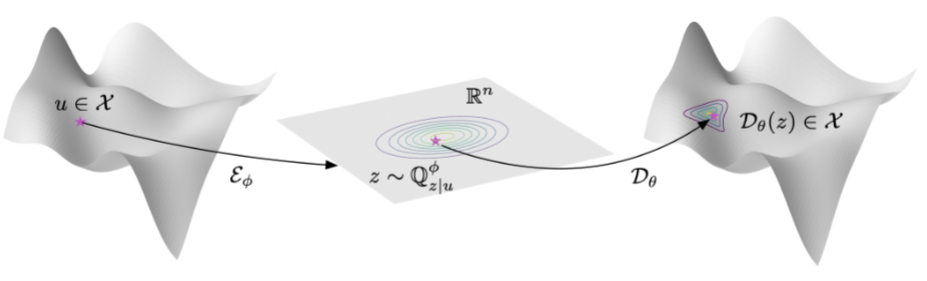
\includegraphics[width=0.5\linewidth]{fig.png}
    \caption{Figure 1 from VANO.}
    \label{fig:vano}
\end{figure}


\section{Detailed Plan for the Project}

Our plan henceforth is to implement VANO in Haiku \cite{haiku2020github}, a deep learning library built on top of Jax. Jax is a numerical computing library that enables ad-hoc XLA pre-compilation of functions, including computing their gradients, Hessians, etc, which makes training machine learning models fast and efficient.

Once we have the VANO architecture ready, we will attempt recreate some, if not all, of the results from the paper on the given benchmarks: (1) a Gaussian Random Field, (2) the Cahn-Hilliard partial differential equation system and (3) the real world InSAR interferogram dataset. It is worth mentioning that (3) is publicly accessible \cite{rahman2022generative}, which means (1) and (2) will have to be constructed manually, (1) being at least more trivial to generate than (2). As mentioned previously, we have collected a plethora of other operator learning datasets from \cite{Lu_2022} (\ref{sec:dataset}), on which we plan to evaluate VANO so that we test the model on a diverse set of cases in order to supplement those from the VANO paper. 


We will also compare VANO against existing operator learning models (DeepONets and FNOs) in our experiments. The relevant metrics we will track and analyze are training loss over iterations, relative error and mean squared error on the training and test sets, inference times on both training and test sets, convergence time (total wall clock time to reach the lowest training loss), and the number of epochs to convergence. These metrics will give us strong intuition on the strengths and weaknesses of the different operator learning models in machine learning on various datasets.

One of the other interesting applications of a VAE is tinkering with the learned latent distribution. It would be interesting to visually compare different generated output functions sampled from the encoded latent distribution of a given input function to see how they compare with one another, i.e. if they are different in some intuitive way.

Our code base can be found at the following github link: \url{https://github.com/mwl10/generative_nos}. 

\bibliography{ref}
\end{document}
\endinput
